\section{Signal Modeling}\label{sec:ciSig}

Although the results of this search can be interpreted for multiple signal models, the model of most interest is that of the \llqq contact interactions.
Contact interactions are described by the Lagrangian in Equation \ref{eqn:ciLagrangian}.
There are five free parameters: the characteristic energy scale \lam, and the parameters $\eta_\text{LL}$, $\eta_\text{RR}$, $\eta_\text{LR}$, and $\eta_\text{RL}$.
The model is simplified by selecting one $\eta_{ij}=\pm1$ for $i,j\in[\text{L,R}]$, and setting the rest as zero.
This describes a model where only one chiral coupling is present, dubbed ``$ij$''.
Furthermore, if $\eta_{ij}=-1$ then the interference of the coupling with the Standard Model is constructive, while if $\eta_{ij}=+1$, it is destructive.
Therefore, eight signal models are considered: four chiral combinations, times two interference patterns, as shown in the table below.
\begin{center}
\begin{tabular}{l l l}
  \toprule
  Lepton channel & Interference & Chirality \\
  \midrule
  $ee$ & Constructive & LL, RL, LR, RR \\
  $ee$ & Destructive & LL, RL, LR, RR \\
  $\mu\mu$ & Constructive & LL, RL, LR, RR \\
  $\mu\mu$ & Destructive & LL, RL, LR, RR \\
  \bottomrule
\end{tabular}
\end{center}


% Generating the TH1 histograms
Signal shapes for the full \mll distribution are modeled using a matrix-element reweighting~\cite{EXOT-2016-05} of the leading-order (LO) DY samples.
This reweighting includes the full interference between the non-resonant signal and the background DY process.
The weight function is the ratio of the analytical matrix-elements of the full CI (including the DY component) and the DY process only, both at LO.
It takes as an input the generated dilepton mass at Born level before FSR, the incoming quarks' flavor and the CI model parameters (\lam, chirality states, and the interference structure).
These weights are applied to the LO DY events to transform these into the CI signal shapes, in steps of $2$~TeV between $\Lambda=12$~TeV and $\Lambda=100$~TeV.
Dilepton mass-dependent higher-order QCD production corrections for the signals are computed with the same methodology as for the DY background, correcting from LO to NNLO.
Similarly, electroweak corrections for the signals are applied in the CI reweighting along with the interference effects, correcting from LO to NLO.
% The ratios of the CI reweighted \mll distributions to the nominal \mll shape are shown for LL chirality in Figure \ref{fig:ciSignalRatiosToNominal}.
The CI component of the signal shape (direct production and interference) is referred to as the \emph{signal}. This is produced by subtracting the LO DY shape from the combined DY+CI shape.
The full \mll signal shapes are shown along with the background function in Figure \ref{fig:ciSignalShape}.

\afterpage{
\begin{figure}[hb]
\begin{center}
\subfloat[][]{{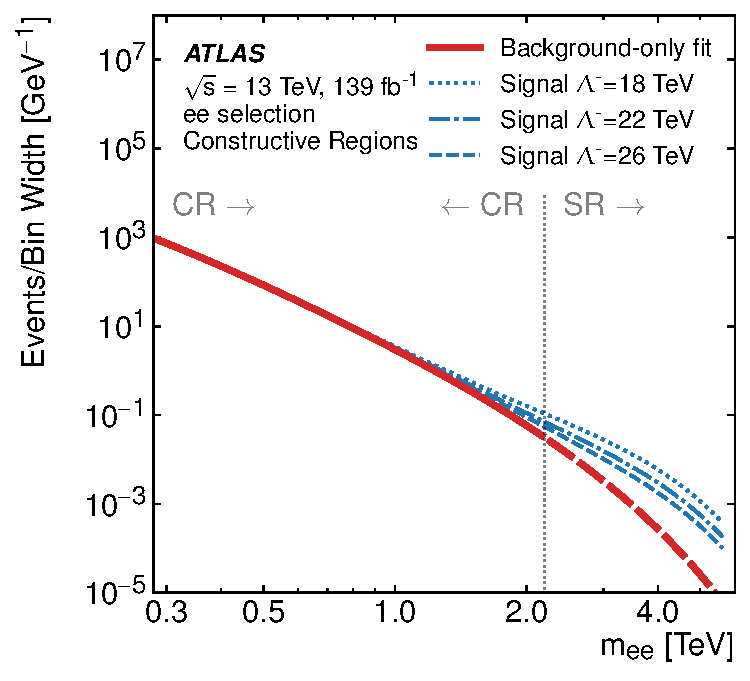
\includegraphics[width=0.45\textwidth]{figures/ci/sigRatio/figaux_01a.pdf}}}
\subfloat[][]{{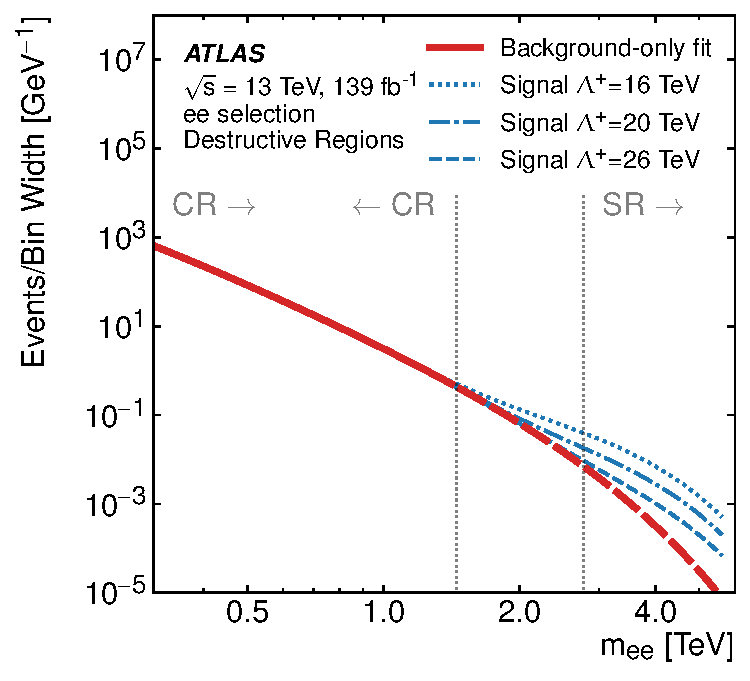
\includegraphics[width=0.45\textwidth]{figures/ci/sigRatio/figaux_01b.pdf}}} \\
\subfloat[][]{{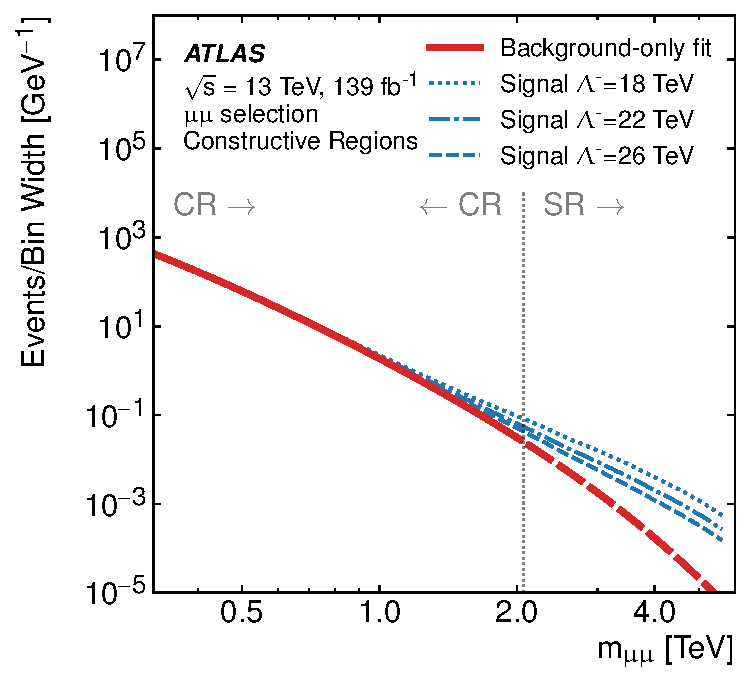
\includegraphics[width=0.45\textwidth]{figures/ci/sigRatio/figaux_02a.pdf}}}
\subfloat[][]{{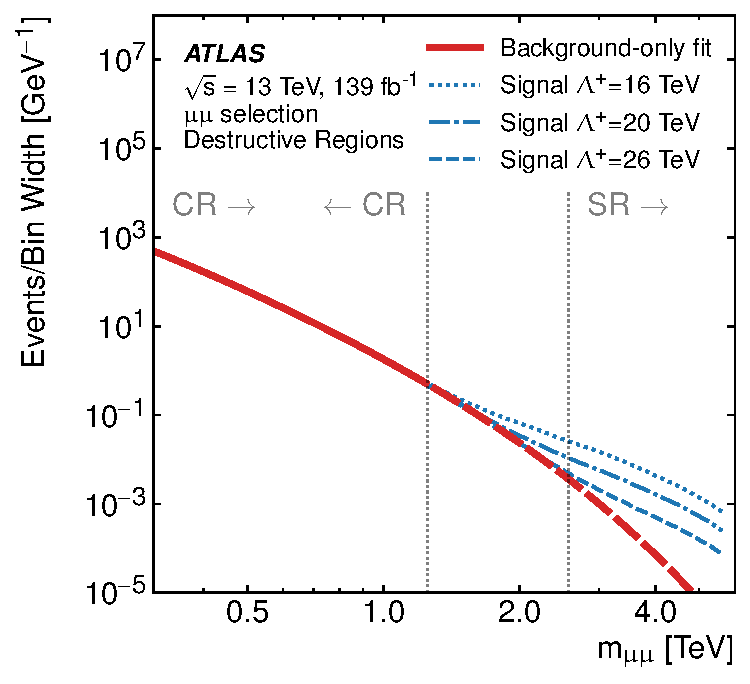
\includegraphics[width=0.45\textwidth]{figures/ci/sigRatio/figaux_02b.pdf}}}
\caption{Signal and background only shapes for the \ee channel (top) and \mm channel (bottom). Constructive signal shapes are shown on the left, and destructive signal shapes are shown on the right. The background shape is derived from a fit of the background model's functional form to the data in the control region. The signal shapes are signal shapes described in the text, added to the background model fit to data.}
\label{fig:ciSignalShape}
\end{center}
\end{figure}
\clearpage
}

% Morphing
The CI signal samples are generated in discrete steps, but it is useful to have a continuous signal description for arbitrary \lam.
Several RooFit classes were developed to interpolate between the generated CI samples smoothly.
\begin{itemize}
    \item \textbf{RooAbsPdf} handles the shape, depending on \lam. This takes a number of input histograms. It interpolates between the histograms' bins to the nearest \mll and between the closest histograms to a particular \lam.
    \item \textbf{RooRealVar} handles the normalization of the signal shape, depending on \lam.
\end{itemize}
The advantage of this implementation is that the signal model is compatible with all the fitting and limit setting operations performed with RooFit.
The \lam parameter can be adjusted by RooFit, resulting in a smoothly changing PDF and normalization.

% Morphing interpolations
The PDF class performs two interpolations.
First, a linear interpolation is made between the histogram bin values.
This is used to prevent RooFit from getting stuck while calculating the integral of the PDF (when RooFit sees a discontinuity, it tends to get stuck looking for a delta function).
The second interpolation is between \lam values for different histograms.
This procedure is called \emph{morphing}.

As opposed to a model with a floating signal strength $\mu$, the utility of this morphed model is clear in these plots.
For constructive cases, the signal shapes are roughly the same for different \lam.
In this case, there is an approximate relationship between $\mu$ and \lam, so a fit using a fixed $\Lambda=20$ TeV where $\mu$ is adjusted could represent, for example, $\Lambda=30$ TeV.
This is not the case for the destructive case, as seen in the figures.
The cross over where the signal contribution becomes negative changes with \lam, while it would not change when scaling a given model by $\mu$.
In fact, there are also subtle differences between the constructive signal shapes.
Using the model in terms of \lam makes the constructive signal model more accurate.

Another motivation for using \lam as the parameter-of-interest (POI) in the S+B model is that this maps more directly onto the physics of the problem.
When searching for a resonance, it is natural that the POI be the signal strength $\mu$.
This is both the parameter dictating the strength of the signal and the  parameter on which limits are set.
Likewise, when searching for a contact interaction, the signal's strength is determined by \lam, and the analysis interest is in setting limits on \lam.
There is no physical motivation for a $\Lambda=20$ TeV model scaled by $\mu>1$ to try to represent $\Lambda=10$ TeV. Instead, the morphed signal model allows limits to be set on \lam directly.

Several examples of the morphed signal model are shown in Figure \ref{fig:ciSigModelTemplateCompMm} (muon channel) and Figure \ref{fig:ciSigModelTemplateCompEe} (electron channel).


\afterpage{
\begin{figure}[htp]
\centering
\subfloat[][]{{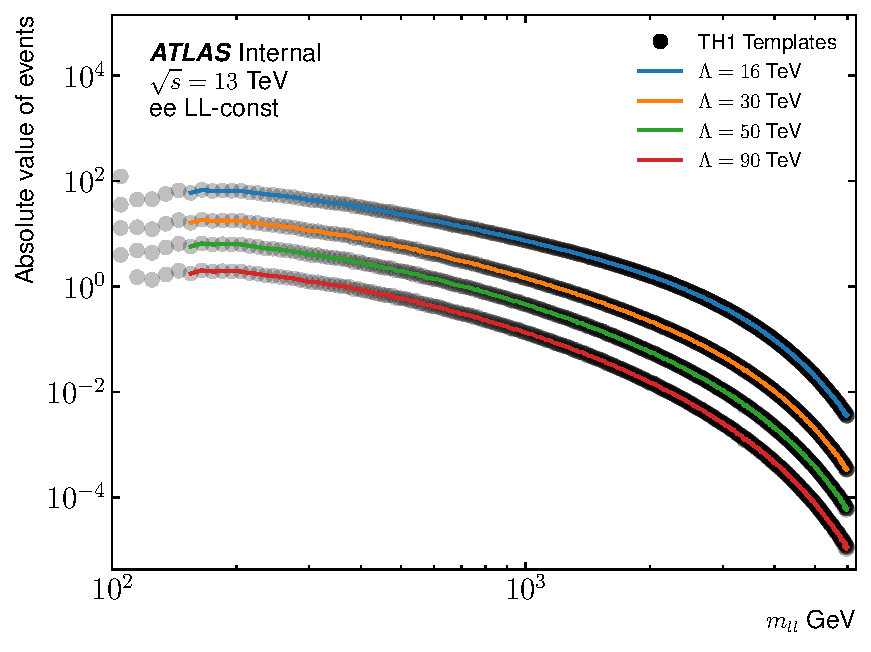
\includegraphics[width=0.40\textwidth]{figures/ci/morphedPdf/sigComp-const-LL-ee.pdf}}}
\subfloat[][]{{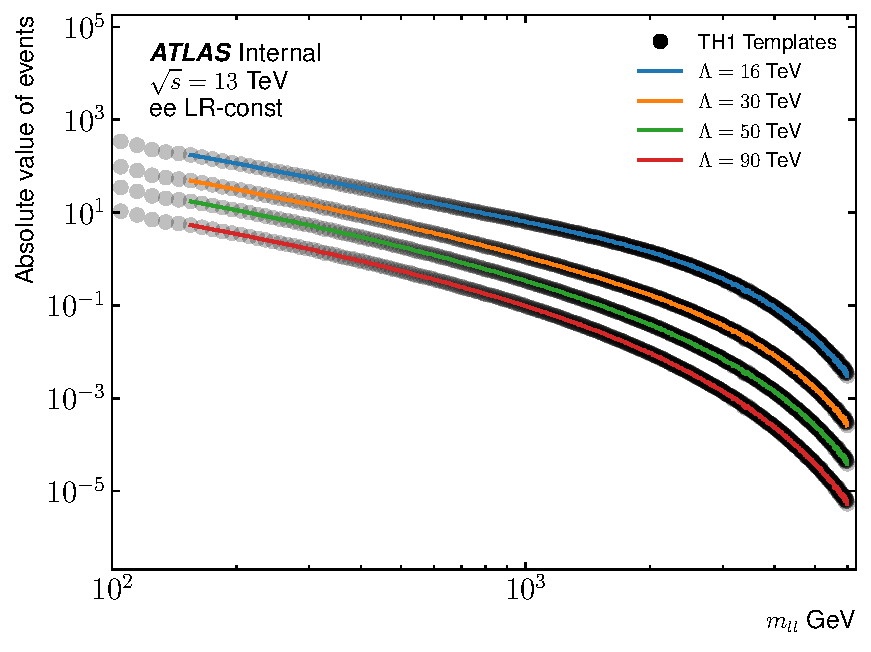
\includegraphics[width=0.40\textwidth]{figures/ci/morphedPdf/sigComp-const-LR-ee.pdf}}} \\
\vspace{-0.3em}
\subfloat[][]{{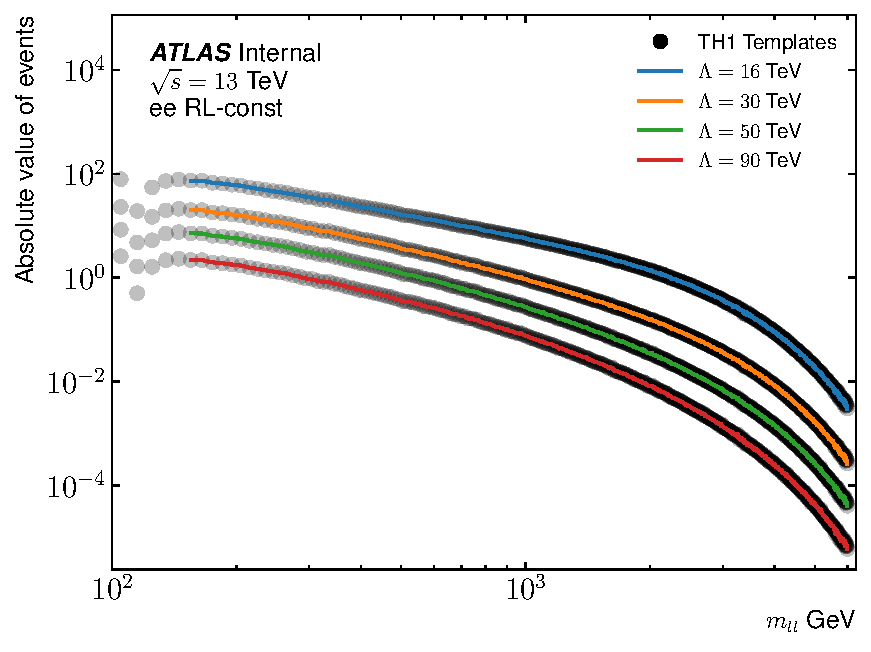
\includegraphics[width=0.40\textwidth]{figures/ci/morphedPdf/sigComp-const-RL-ee.pdf}}}
\subfloat[][]{{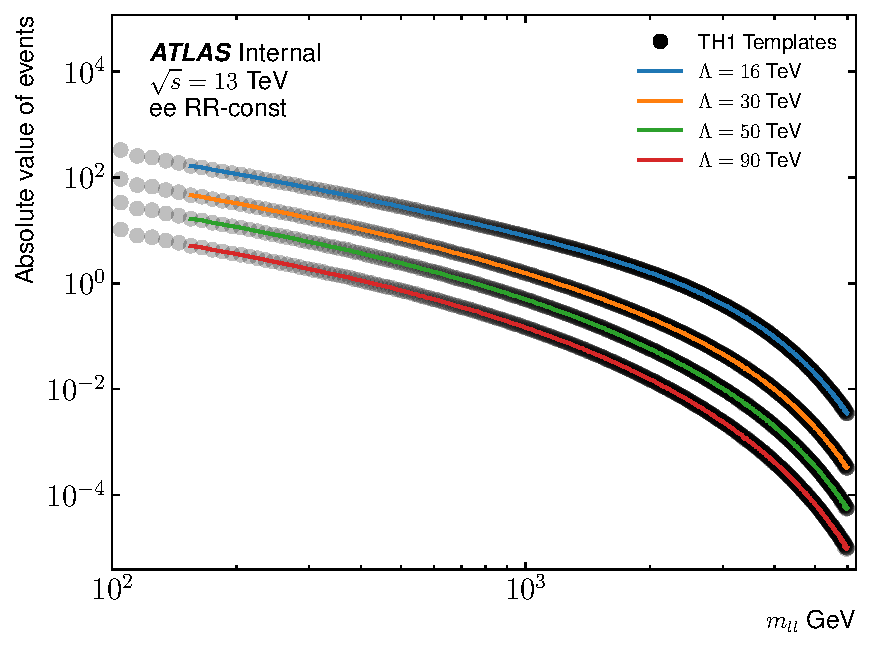
\includegraphics[width=0.40\textwidth]{figures/ci/morphedPdf/sigComp-const-RR-ee.pdf}}} \\
\vspace{-0.3em}
\subfloat[][]{{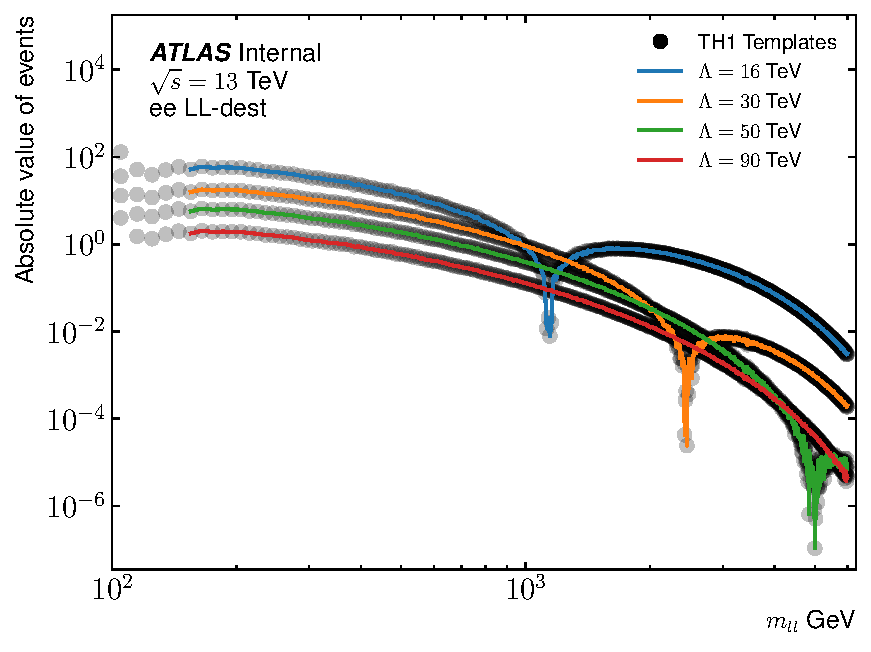
\includegraphics[width=0.40\textwidth]{figures/ci/morphedPdf/sigComp-dest-LL-ee.pdf}}}
\subfloat[][]{{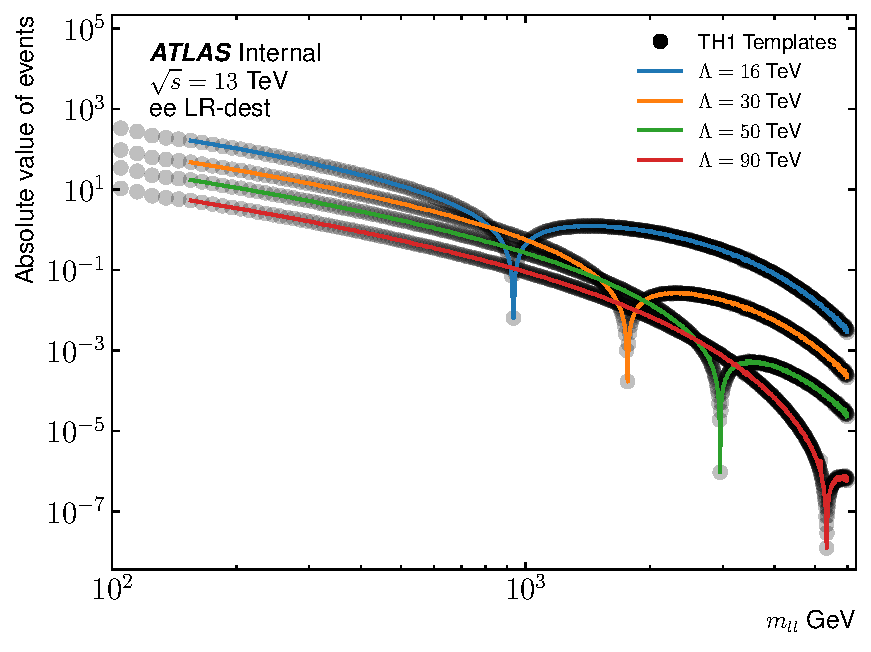
\includegraphics[width=0.40\textwidth]{figures/ci/morphedPdf/sigComp-dest-LR-ee.pdf}}} \\
\vspace{-0.3em}
\subfloat[][]{{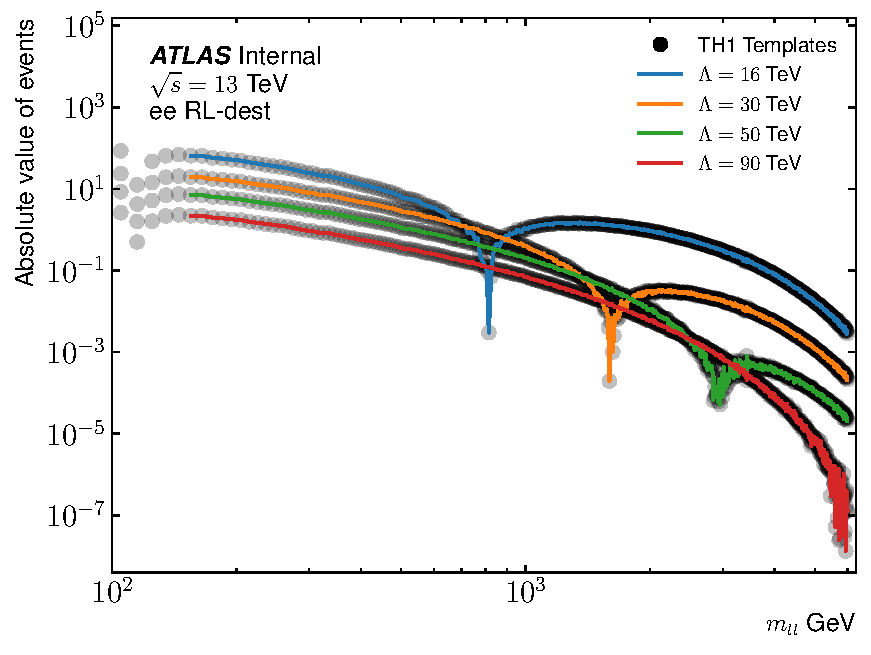
\includegraphics[width=0.40\textwidth]{figures/ci/morphedPdf/sigComp-dest-RL-ee.pdf}}}
\subfloat[][]{{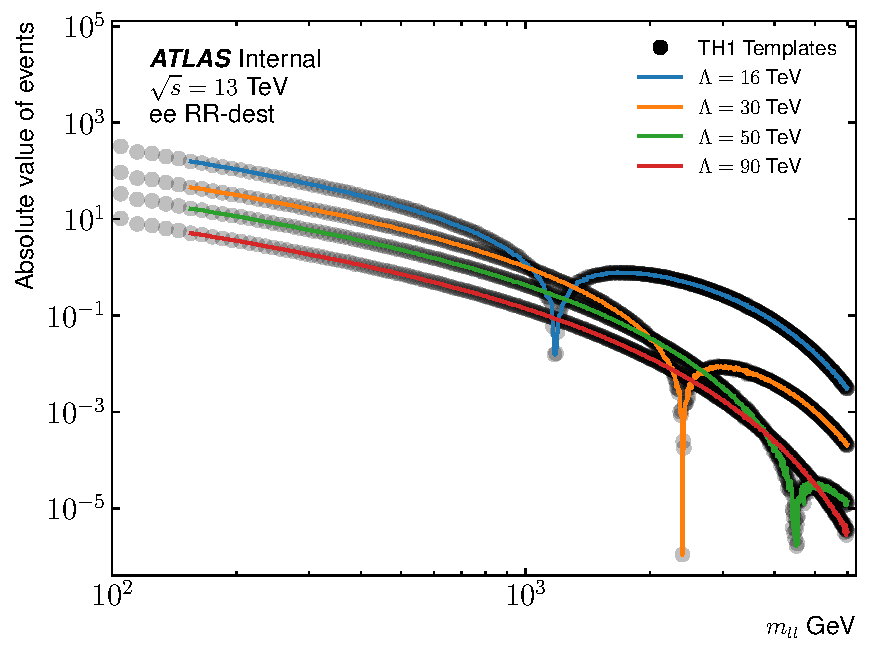
\includegraphics[width=0.40\textwidth]{figures/ci/morphedPdf/sigComp-dest-RR-ee.pdf}}}
\caption{Comparison between the morphed signal model (colored) and the underlying TH1 templates (black) for \textbf{constructive} signal shapes for chiralities LL (a), LR (b), RL (c), RR (d), and for \textbf{destructive} signal shapes for chiralities LL (e), LR (f), RL (g), RR (h) for the $ee$ channel. This comparison is both of the shape and normalization of the morphed signal model. Note that since these show the negative component of the destructive signal on a log scale plot, the absolute value of the template has been taken. The low mass part of the signal shape is really negative, while the high mass part is positive.}
\label{fig:ciSigModelTemplateCompEe}
\end{figure}
\clearpage
}

\afterpage{
\begin{figure}[htp]
\centering
\subfloat[][]{{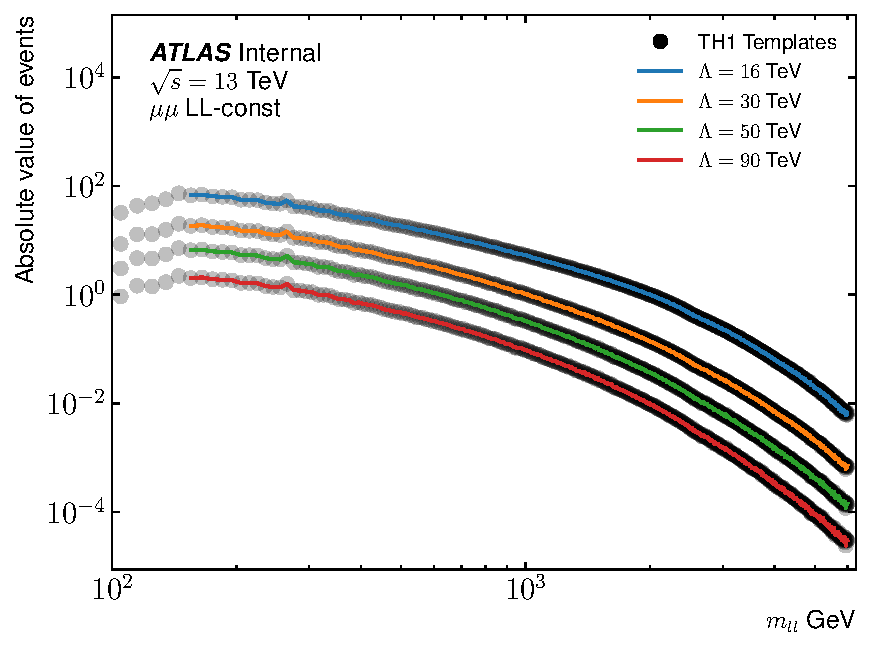
\includegraphics[width=0.40\textwidth]{figures/ci/morphedPdf/sigComp-const-LL-mm.pdf}}}
\subfloat[][]{{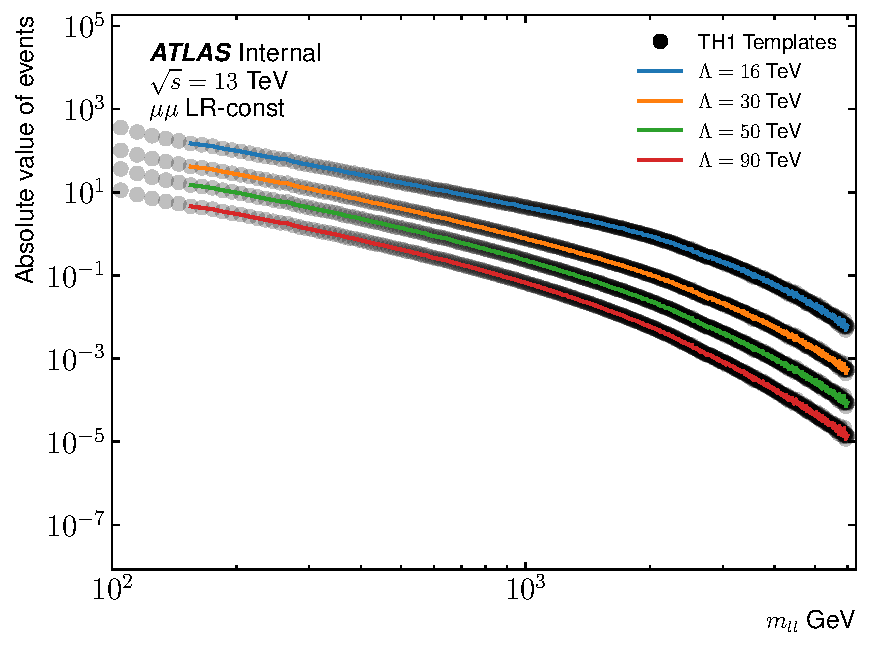
\includegraphics[width=0.40\textwidth]{figures/ci/morphedPdf/sigComp-const-LR-mm.pdf}}} \\
\vspace{-0.3em}
\subfloat[][]{{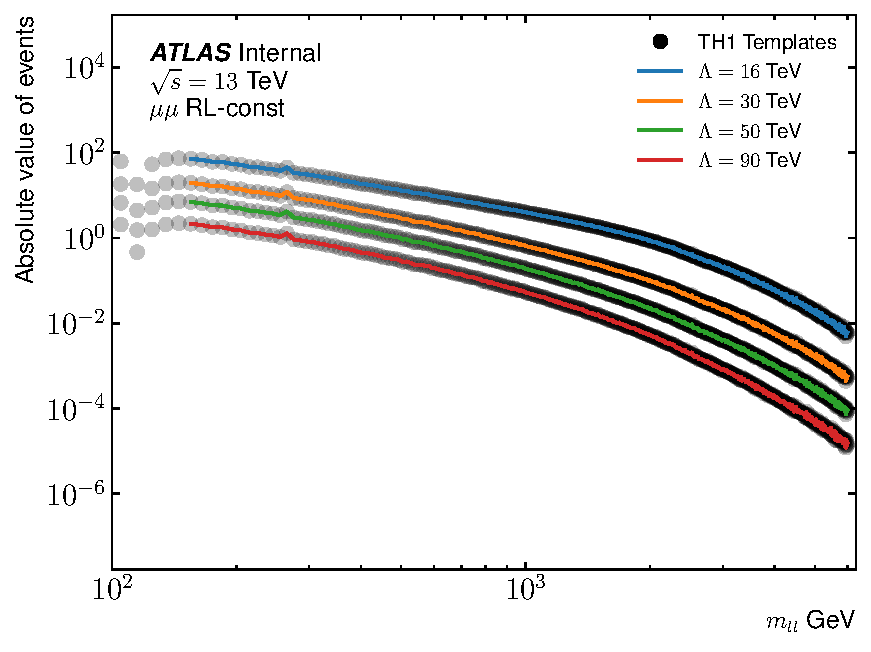
\includegraphics[width=0.40\textwidth]{figures/ci/morphedPdf/sigComp-const-RL-mm.pdf}}}
\subfloat[][]{{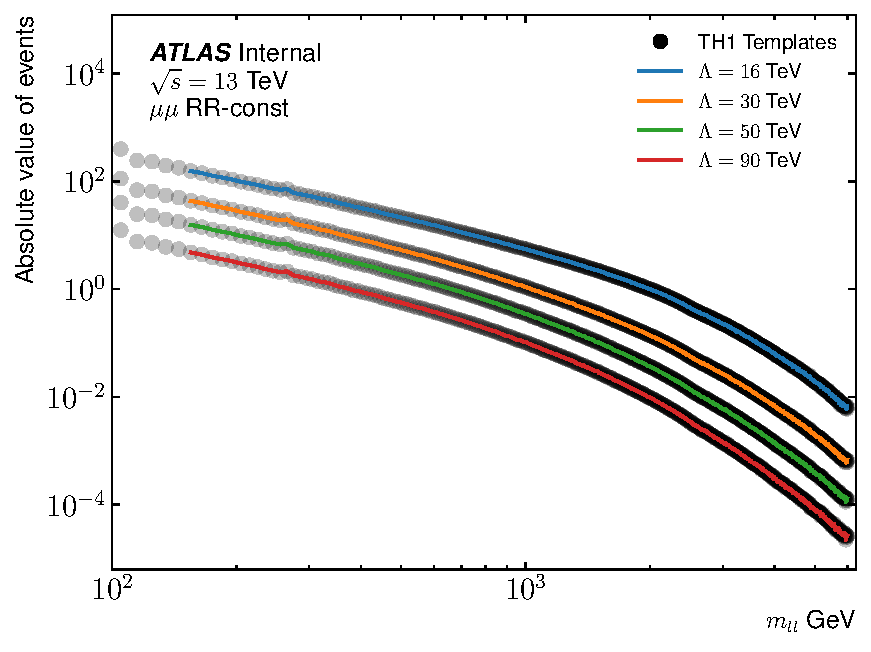
\includegraphics[width=0.40\textwidth]{figures/ci/morphedPdf/sigComp-const-RR-mm.pdf}}} \\
\vspace{-0.3em}
\subfloat[][]{{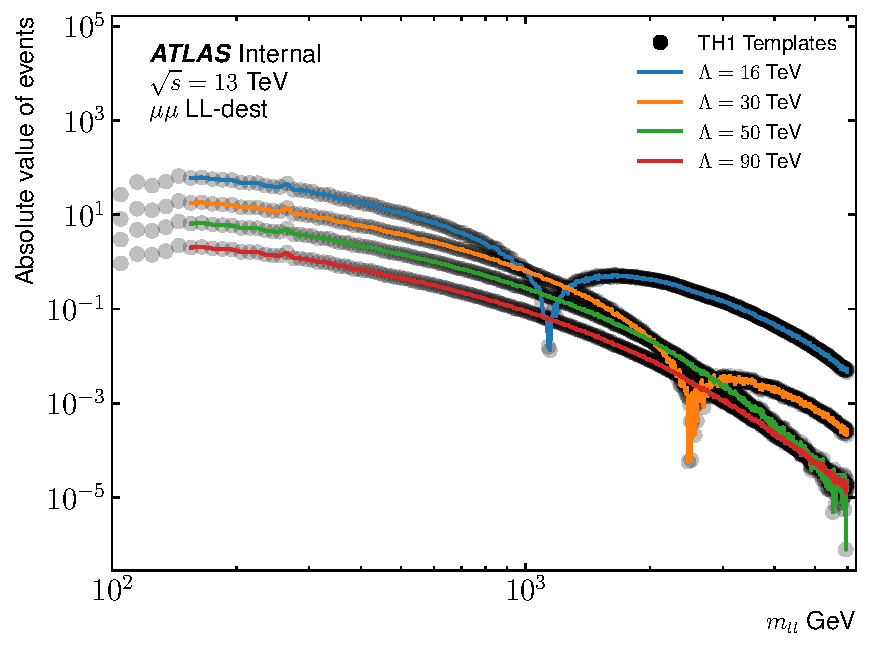
\includegraphics[width=0.40\textwidth]{figures/ci/morphedPdf/sigComp-dest-LL-mm.pdf}}}
\subfloat[][]{{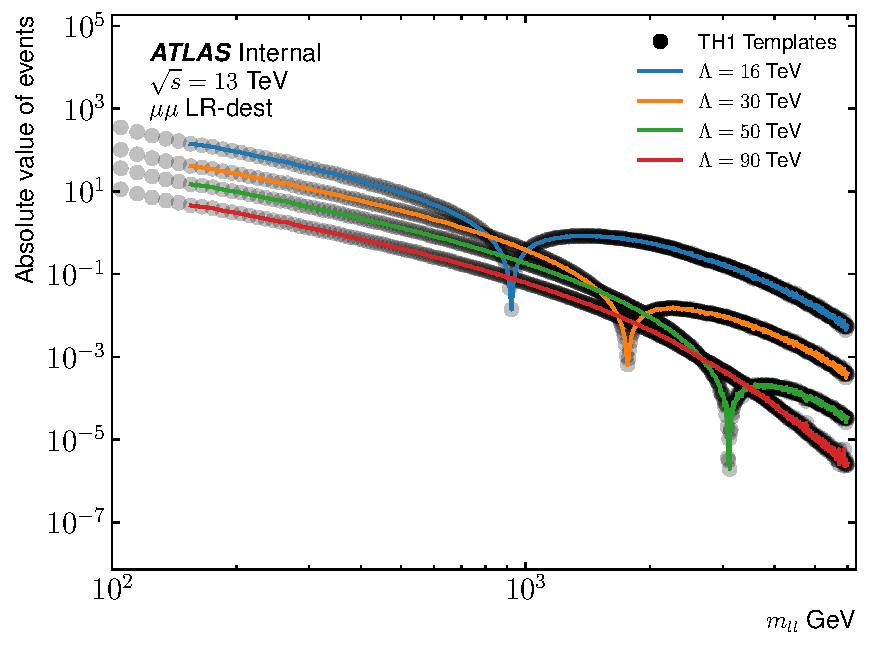
\includegraphics[width=0.40\textwidth]{figures/ci/morphedPdf/sigComp-dest-LR-mm.pdf}}} \\
\vspace{-0.3em}
\subfloat[][]{{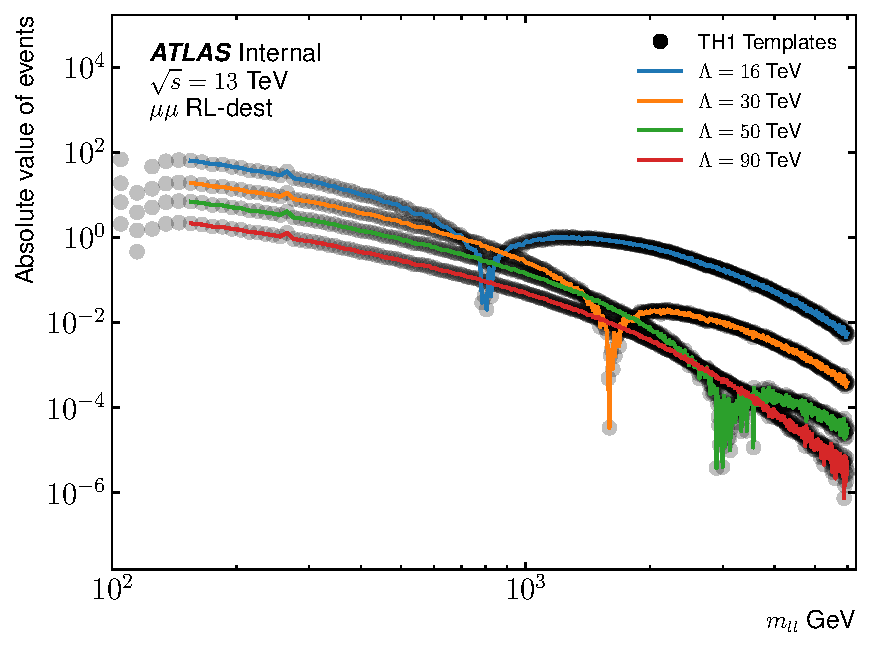
\includegraphics[width=0.40\textwidth]{figures/ci/morphedPdf/sigComp-dest-RL-mm.pdf}}}
\subfloat[][]{{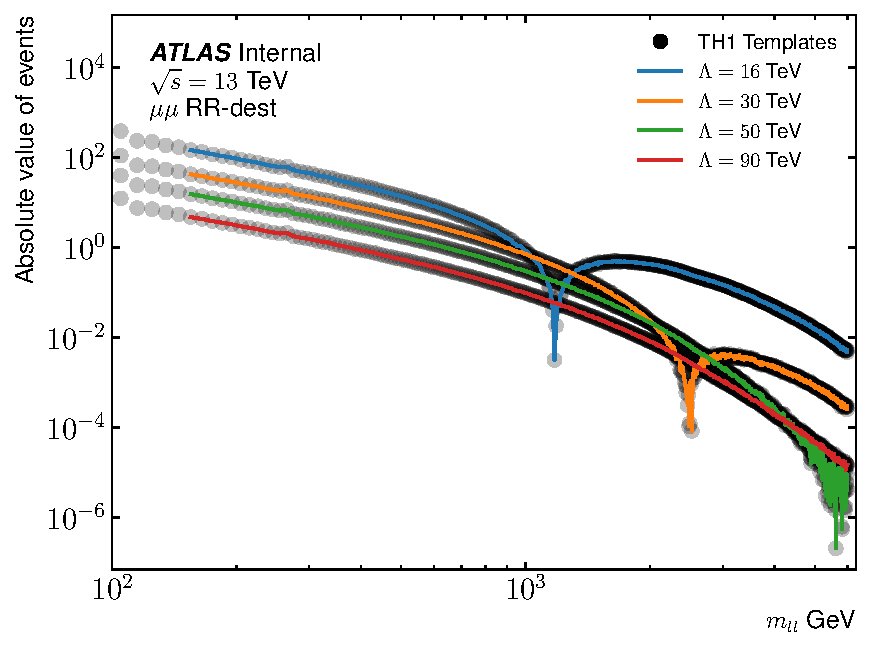
\includegraphics[width=0.40\textwidth]{figures/ci/morphedPdf/sigComp-dest-RR-mm.pdf}}}
\caption{Comparison between the morphed signal model (colored) and the underlying TH1 templates (black) for \textbf{constructive} signal shapes for chiralities LL (a), LR (b), RL (c), RR (d), and for \textbf{destructive} signal shapes for chiralities LL (e), LR (f), RL (g), RR (h) for the $\mu\mu$ channel. This comparison is both of the shape and normalization of the morphed signal model. Note that since these show the negative component of the destructive signal on a log scale plot, the absolute value of the template has been taken. The low mass part of the signal shape is really negative, while the high mass part is positive.}
\label{fig:ciSigModelTemplateCompMm}
\end{figure}
\clearpage
}

% S+B model
The full signal shape is used in an extension of the background functions, Equations \ref{eqn:ciBkgEe} and \ref{eqn:ciBkgMm}.
A signal shape, based on the morphed CI signals, is added to the background-only shape, producing an S+B functional form:
\begin{align}
\label{eqn:ciSB}
f_\textrm{s+b}(m_{\ell\ell},\Lambda) = N_\textrm{b}\cdot f_\textrm{b}(m_{\ell\ell}) + N_\textrm{s}(\Lambda)\cdot f_\textrm{s}(m_{\ell\ell},\Lambda),
\end{align}
where $f_\textrm{s}(m_{\ell\ell},\Lambda)$ is the signal probability density function and $N_\textrm{s}(\Lambda)$ is the number of signal events in the CR.
Both $f_\textrm{s}(m_{\ell\ell},\Lambda)$ and $N_\textrm{s}(\Lambda)$ are determined by the morphed CI signals.
The parameter $N_\textrm{b}$ is the number of background events in the CR with the constraint $N_\textrm{b}+N_\textrm{s}(\Lambda)=N_\textrm{CR}$.
The functional form of Equation \ref{eqn:ciSB} is useful because, even in when a large signal is present in the CR, the $N_\textrm{s}(\Lambda)\cdot f_\textrm{s}(m_{\ell\ell},\Lambda)$ term absorbs it.
This leaves the background component undeflected by the presence of a signal.
This property is validated through signal-injection tests detailed in Appendix \ref{sec:ciLinearity}.
This makes Equation \ref{eqn:ciSB} a useful tool to constrain the degree to which the background-only functions (\ref{eqn:ciBkgEe} and \ref{eqn:ciBkgMm}) have been deflected by the presence of a signal in the CR.
This will be further discussed, along with other systematic uncertainties, in Section \ref{sec:ciSyst}.

% The real signal: integral in the SR's
The signal model described up until this point is the differential signal shape in the invariant-mass distribution.
However, the analysis of signal regions considers only the number of events in the region as a function of \lam.
Figure \ref{fig:ciNSigInSr} shows the number of events in each signal region, predicted by various interference and chirality models.
Of particular interest, the RR and LL models predict more events than the LR and RL models in the constructive case.
This pattern is reversed for constructive models.
This is due to the projection of the two chirality operators (Equation \ref{eqn:chiralOps}) hidden in the left and right-handed fermion fields of the Lagrangian (Equation \ref{eqn:ciLagrangian}).
The pattern of varying multiplicity seen in Figure \ref{fig:ciNSigInSr} will later manifest itself in the strength of limits on various CI models.

\afterpage{
\begin{figure}[htp]
\centering
\subfloat[][]{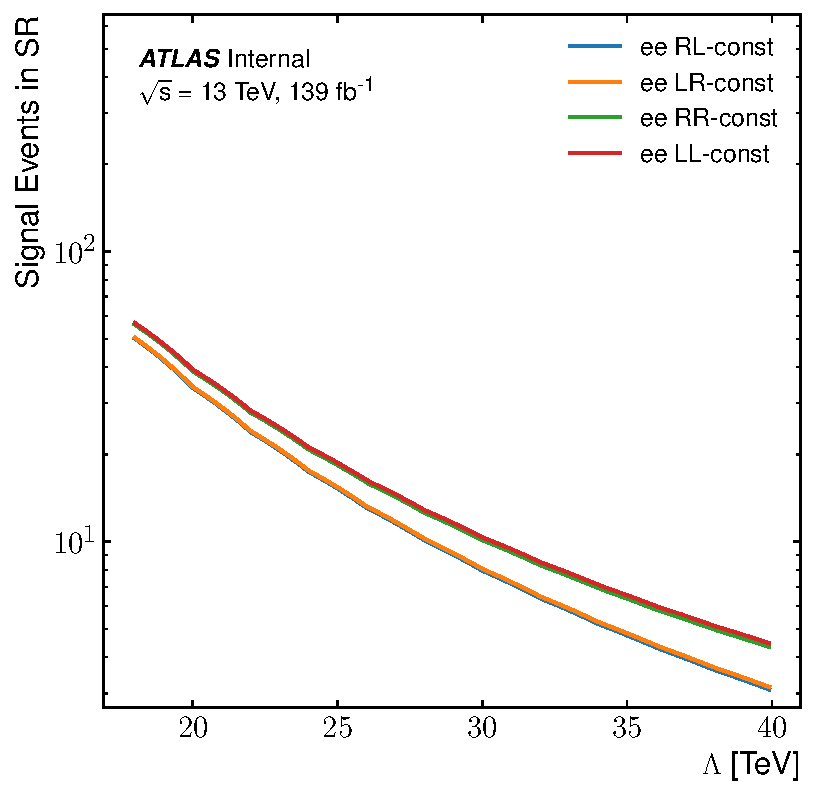
\includegraphics[width=0.449\textwidth]{figures/ci/signalInSr/nSigFunc-ee-const.pdf}}
\subfloat[][]{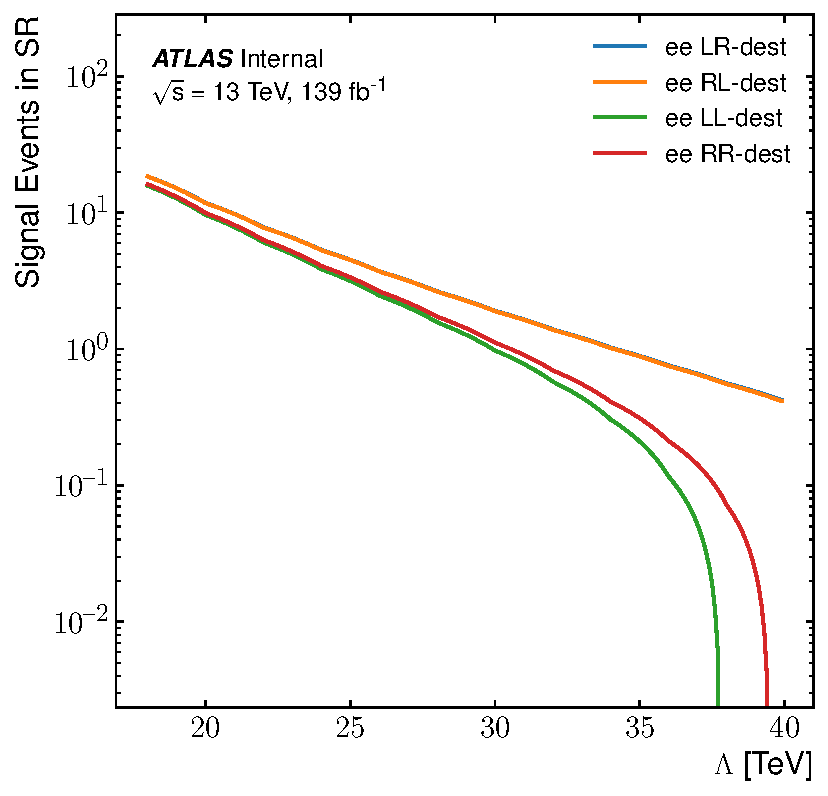
\includegraphics[width=0.449\textwidth]{figures/ci/signalInSr/nSigFunc-ee-dest.pdf}} \\
\subfloat[][]{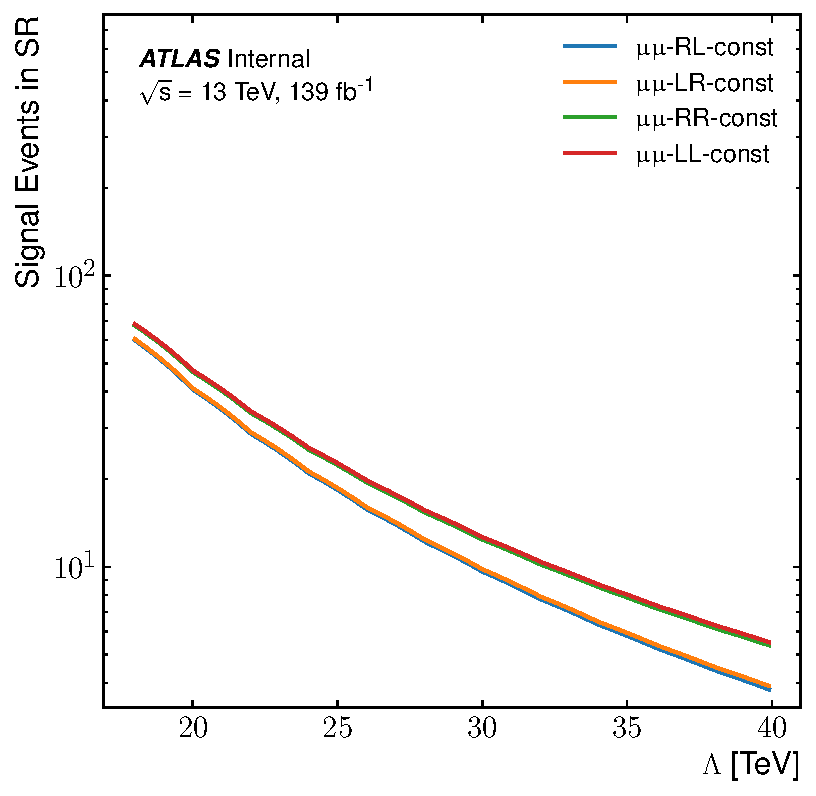
\includegraphics[width=0.449\textwidth]{figures/ci/signalInSr/nSigFunc-mm-const.pdf}}
\subfloat[][]{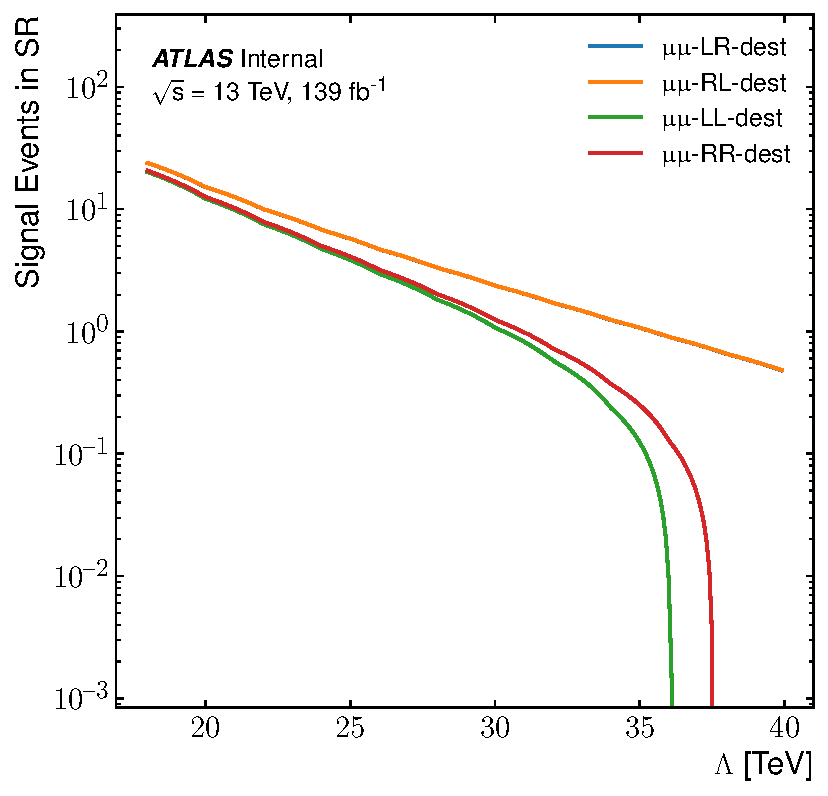
\includegraphics[width=0.449\textwidth]{figures/ci/signalInSr/nSigFunc-mm-dest.pdf}}
\caption{The number of signal events using the morphed model of signal events in each of the four SR's used in the analysis: $ee$-const, $ee$-dest, $\mu\mu$-const, $\mu\mu$-dest in a, b, c, d respectively. Each plot shows the number of signal events as a function of $\Lambda$ for the four chiralities.}
\label{fig:ciNSigInSr}
\end{figure}
\clearpage
}

\afterpage{
\begin{figure}[tb]
\begin{center}
\subfloat[][]{{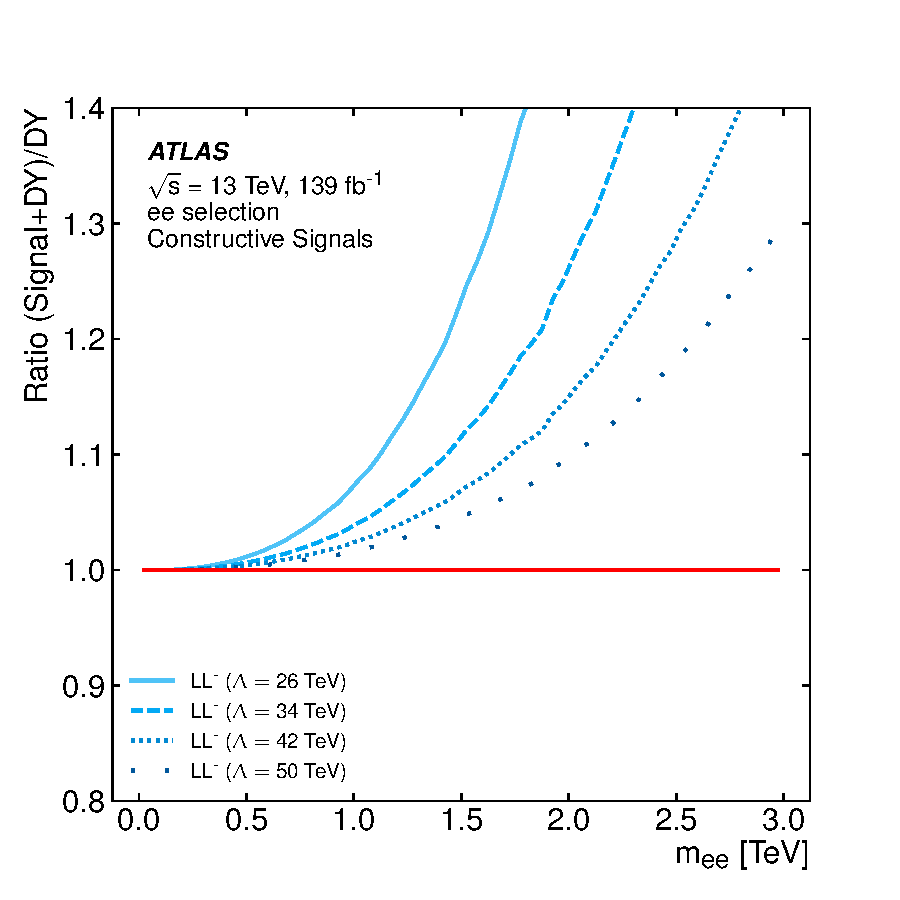
\includegraphics[width=0.45\textwidth]{figures/ci/sigRatio/figaux_04a.pdf}}}
\subfloat[][]{{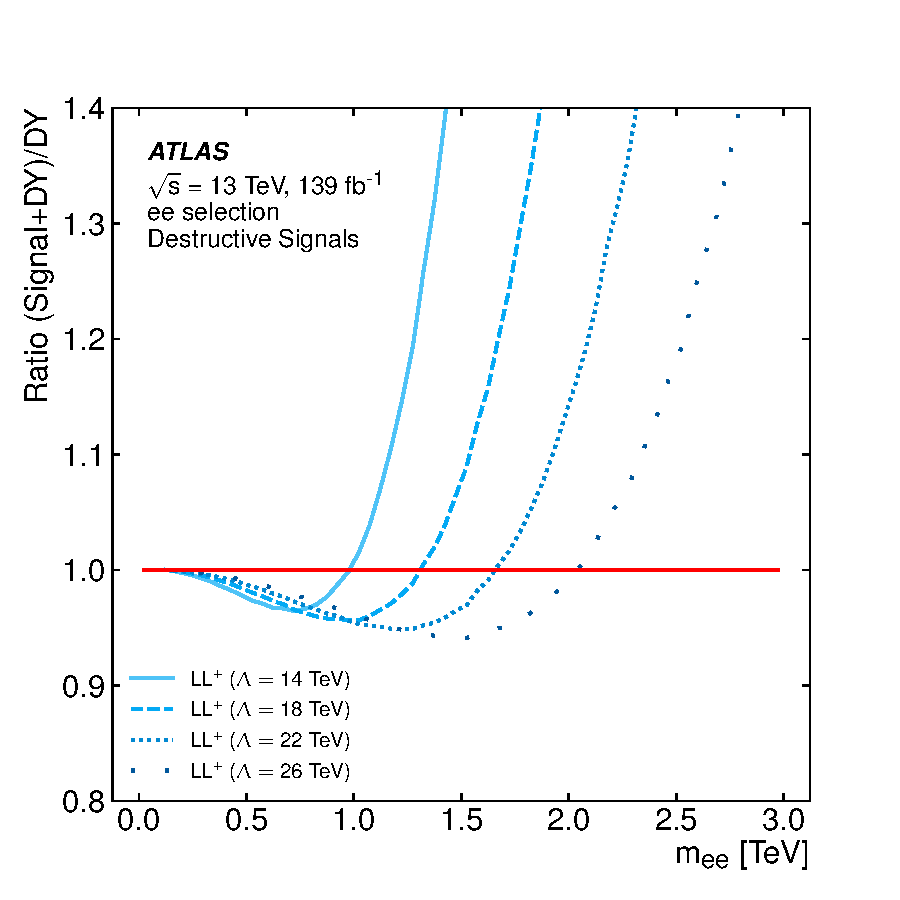
\includegraphics[width=0.45\textwidth]{figures/ci/sigRatio/figaux_04b.pdf}}} \\
\subfloat[][]{{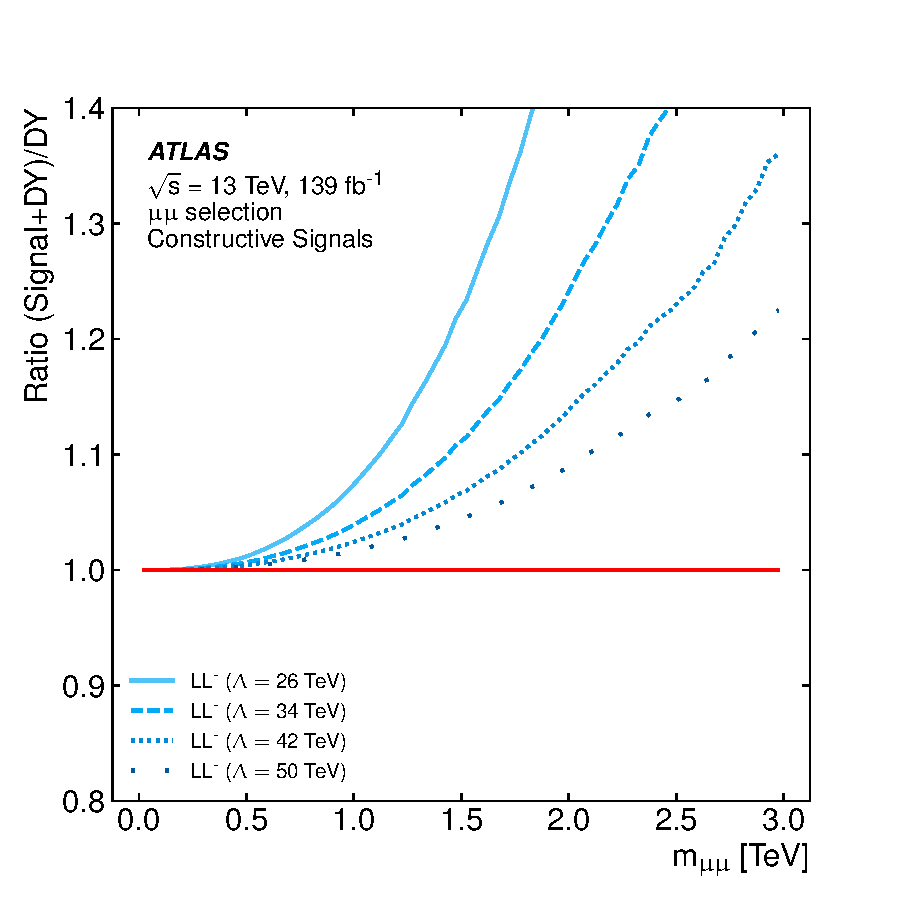
\includegraphics[width=0.45\textwidth]{figures/ci/sigRatio/figaux_04c.pdf}}}
\subfloat[][]{{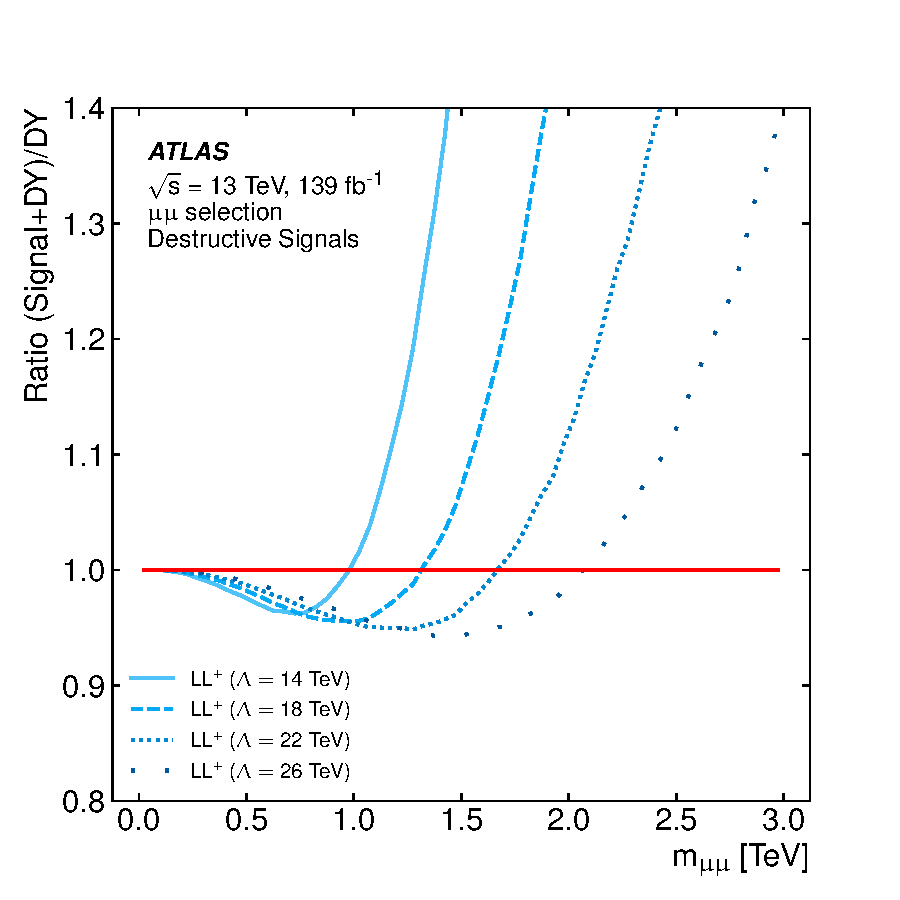
\includegraphics[width=0.45\textwidth]{figures/ci/sigRatio/figaux_04d.pdf}}}
\caption{Signal templates for the CI LL model with constructive (left) and destructive (right) interference for the  dielectron channel is presented for 4 \lam values. The reweighted templates are produced from the same DY sample, therefore the same statistical fluctuations of the underlying DY show up in the plots for each \lam. Also, while the ratio tends to blow up at high mass, this is due to the small number of events in the denominator (DY). In the destructive case, the $\Lambda=30$ TeV signal is still primarily destructive at 2 TeV, but it also has a constructive component at $\approx2.5$ TeV.}
\label{fig:ciSignalRatiosToNominal}
\end{center}
\end{figure}
\clearpage
}
